% 2011 年四川卷文科第 21 题：椭圆 x^2/4+y^2=1（即 a=2、b=1），顶点 A(2,0)、B(-2,0)，
%   C(0,1)，过 C 的直线 l 与椭圆交于另一点 D，交 x 轴于 P，直线 AC 与 BD 交于 Q。
% 来源 PDF：普通高考/2011/2011四川文.pdf，SHA-256 9df4a6b69bb06bfab2f7d7ee0e7fcc50ae547f226260996d7a060c31ad14e64a。
% 原页：第 2 页（A3 三栏）第 2 栏中部，书页码 704。
% 重绘依据：照原页——椭圆横长；B 为左顶点、A 为右顶点，C 在椭圆上、位于 y 轴正半轴；
%   l 自左上斜穿过 C，交 x 轴于 P（O 与 A 之间），再穿过椭圆上一点 D（第四象限）向右下延伸，
%   标号 l 在 D 的右下方；AC 自 A 过 C 向左上延长，BD 自 B 过 D 向右下延长，二者交于 Q（椭圆外右下方）。
%   取 l 的斜率 k=-1，此时 P(1,0)、D(8/5,-3/5)、Q(4,-1)，与原页各点相对位置一致；不按原页比例。
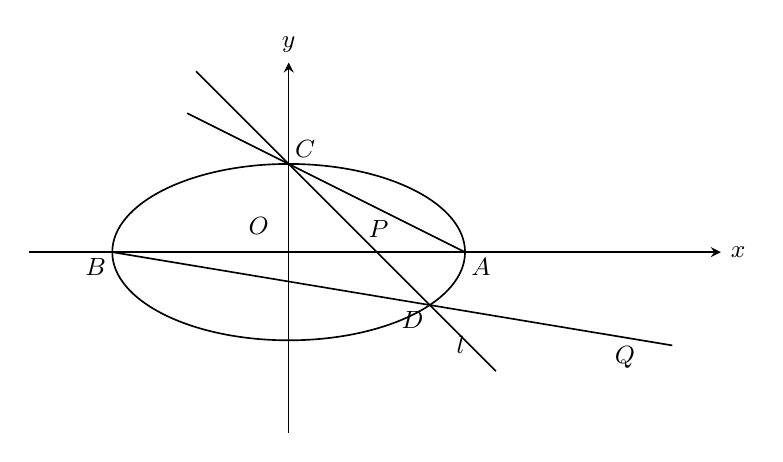
\begin{tikzpicture}[scale=1.12, >=stealth, semithick, font=\small]
  % 坐标轴
  \draw[->] (-2.95,0) -- (4.9,0) node[right] {$x$};
  \draw[->] (0,-2.05) -- (0,2.15) node[above] {$y$};

  % 椭圆
  \draw (0,0) ellipse (2 and 1);

  % 各点
  \coordinate (A) at (2,0);
  \coordinate (B) at (-2,0);
  \coordinate (C) at (0,1);
  \coordinate (D) at (1.6,-0.6);
  \coordinate (P) at (1,0);
  \coordinate (Q) at (4,-1);

  % 直线 l：自左上经 C、P、D 向右下
  \draw (-1.05,2.05) -- (2.35,-1.35);
  % 直线 AC 及其延长
  \draw (A) -- (-1.15,1.575);
  % 直线 BD 及其延长至 Q 并略过
  \draw (B) -- (4.35,-1.058);

  \node at (A) [below right, inner sep=2pt] {$A$};
  \node at (B) [below left, inner sep=2pt] {$B$};
  \node at (C) [above right, inner sep=2pt] {$C$};
  \node at (D) [below left, inner sep=2pt] {$D$};
  \node at (1.02,0.26) {$P$};
  \node at (Q) [below left, inner sep=2pt] {$Q$};
  \node at (-0.34,0.30) {$O$};
  \node at (1.95,-1.05) {$l$};
\end{tikzpicture}
